%!TEX root = ../thesis.tex

\subsection{Blue face subdivision}
\thispagestyle{plain}
\label{ss:subdiv}
  At this point we have a vertically one-sided graph (due to Lemma \ref{lm:topfan:oneSidedREL}) without large topfans except for the locations provided in Lemma \ref{lm:topfan:remainingTopfans}.
  In this section we are going to recolor edges in blue faces to make all of them $d-1$-sided.
  While at the same time not recoloring so many edges above each other that we create a large red face.

  We would like to start at the bottom most face $F$. We can unfortunately no longer use the creation order since the topfan flips may have changed which faces lie above which other faces, the topfan flips may even have introduced new faces.
  Hence, we will have to show that there always is a face $F$  that lies below all untreated faces. That is, the whole top boundary path of $F$ borders faces that are not treated while no part of the bottom boundary path borders such faces.

  \begin{lemma}
    \label{lm:}
    There is a face $F$ such that the whole top boundary path of $F$ borders faces that are not treated while the bottom boundary path does not border such faces.
  \end{lemma}
  \begin{proof}
    Let us first remove all treated faces from $\ext G$ by removing their blue edges and connecting their red edges with $S$.

    Unless there are no faces remaining, and in that case we are finished, there is at least one \emph{splitvertex} (vertex with at least two outgoing blue edges) and one \emph{mergevertex} (vertex with at least two blue incoming edge) along the directed path formed by the vertices adjacent to $\pS$.
    There can be no merges before the first split, nor splits after the last merge.
    Hence, somewhere along the path there is a split followed by a merge.
    This face has a bottom boundary path that is entirely adjacent to $\pS$ after removing treated faces.
    The top boundary path borders untreated faces.
  \end{proof}


  We will recolor some of $F$'s edges if it is too large.
  We then mark the edges on the top boundary path of this face above the recolored edges as \emph{loaded}. This means that we will try to not flip above these edges in future iterations of the algorithm.
  Then we continue with the next face in the creation order.

\mypar{Loads}
  As is mentioned above we will mark some edges with so-called \emph{loads}, we will in the rest of the section refer to these edges as \emph{loaded}.
  The exact use of these loaded edges will become clear in the rest of this section.

  It is important to note that if we load any blue edge we regard any other blue edge sharing at least one vertex with this edge to be loaded as well.
  The occurrence of this phenomenon will be called \emph{putting trough a load}.
  An example can be seen in Figure \ref{fig:subdiv:putTrougLoad} where we flipped the thick edge.
  Hence, we mark $uv$ as loaded and because of putting trough load $uw$ also becomes loaded.

  \begin{figure}[h]
    \centering
    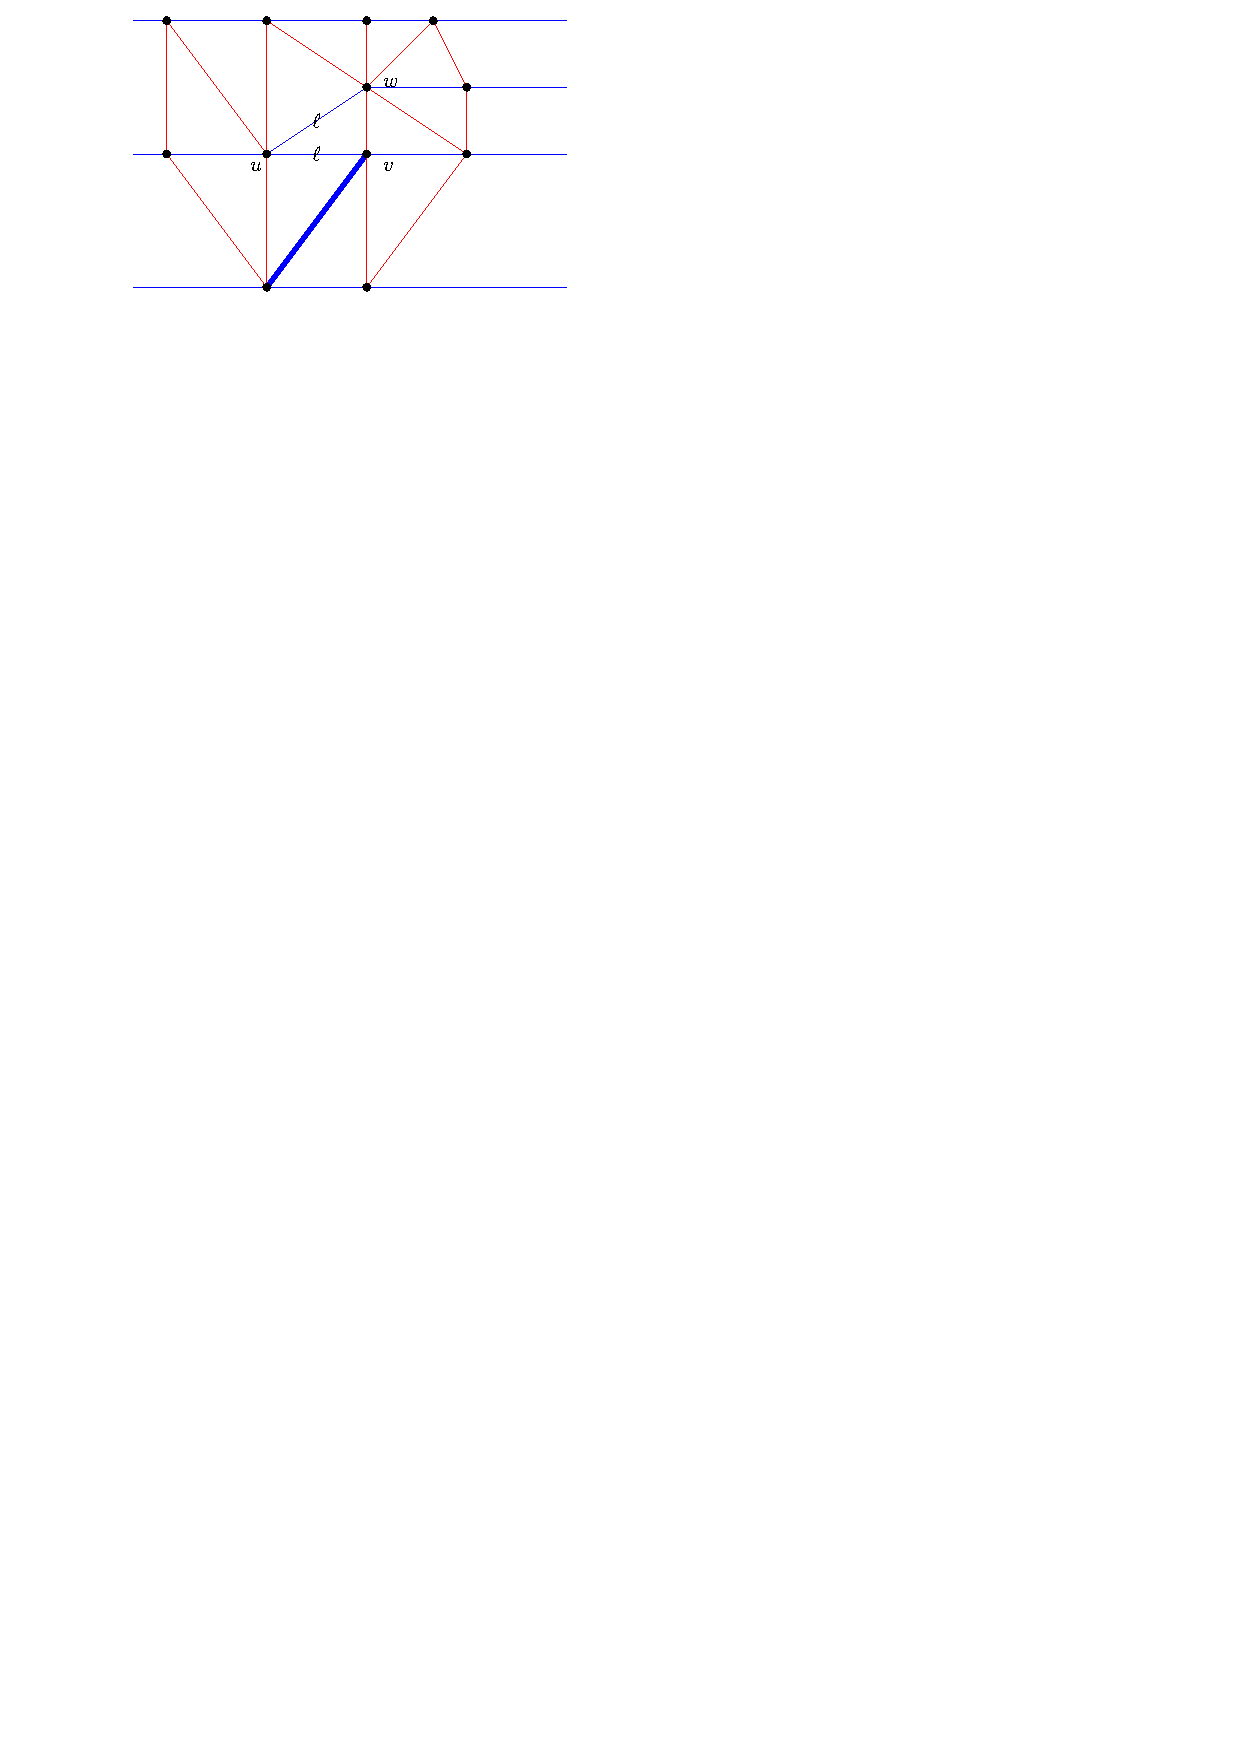
\includegraphics[scale=1]{blueFaceSubdivision/img/puttingTroughLoad.pdf}
    \caption{Putting trough load.}
    \label{fig:subdiv:putTrougLoad}
  \end{figure}


\mypar{Step requirements}
  We flip edges in each face, taking into account loads on the bottom boundary path. Such that

  \begin{enumerate}
    \item We never load the two edges next to a split or merge vertex on the top boundary path.
    \item We never load two adjacent edges on the top boundary path.
  \end{enumerate}

  If we flip edges in line with the step requirements for every face then the following lemma holds for the bottom boundary path for yet untreated faces.

  \begin{lemma}
    \label{lm:}
    On the bottom boundary path of a face we never find two subsequent loaded edges. Even when we put trough loads on splits and merges.
  \end{lemma}
  \begin{proof}
    A single face would never load two subsequent edges. Hence, the only way to get two subsequent loaded edges is using different faces and thus splits and merges.
    However due to never flipping the two edges next to a split or merge we neither get subsequent loaded edges in such a case.
  \end{proof}


\subsubsection{Faces without large topfans in the middle}
  \begin{lemma}
    \label{lm:subdiv:withoutTopfan}
    We can subdivide any blue face without large topfans into $d-1$-sided chunks while obeying the load rules above.
  \end{lemma}

  \begin{proof}
  A worst case example is given in Figure \ref{fig:subdiv:worstCaseWithTopFan}.

  \begin{figure}[b]
    \centering
    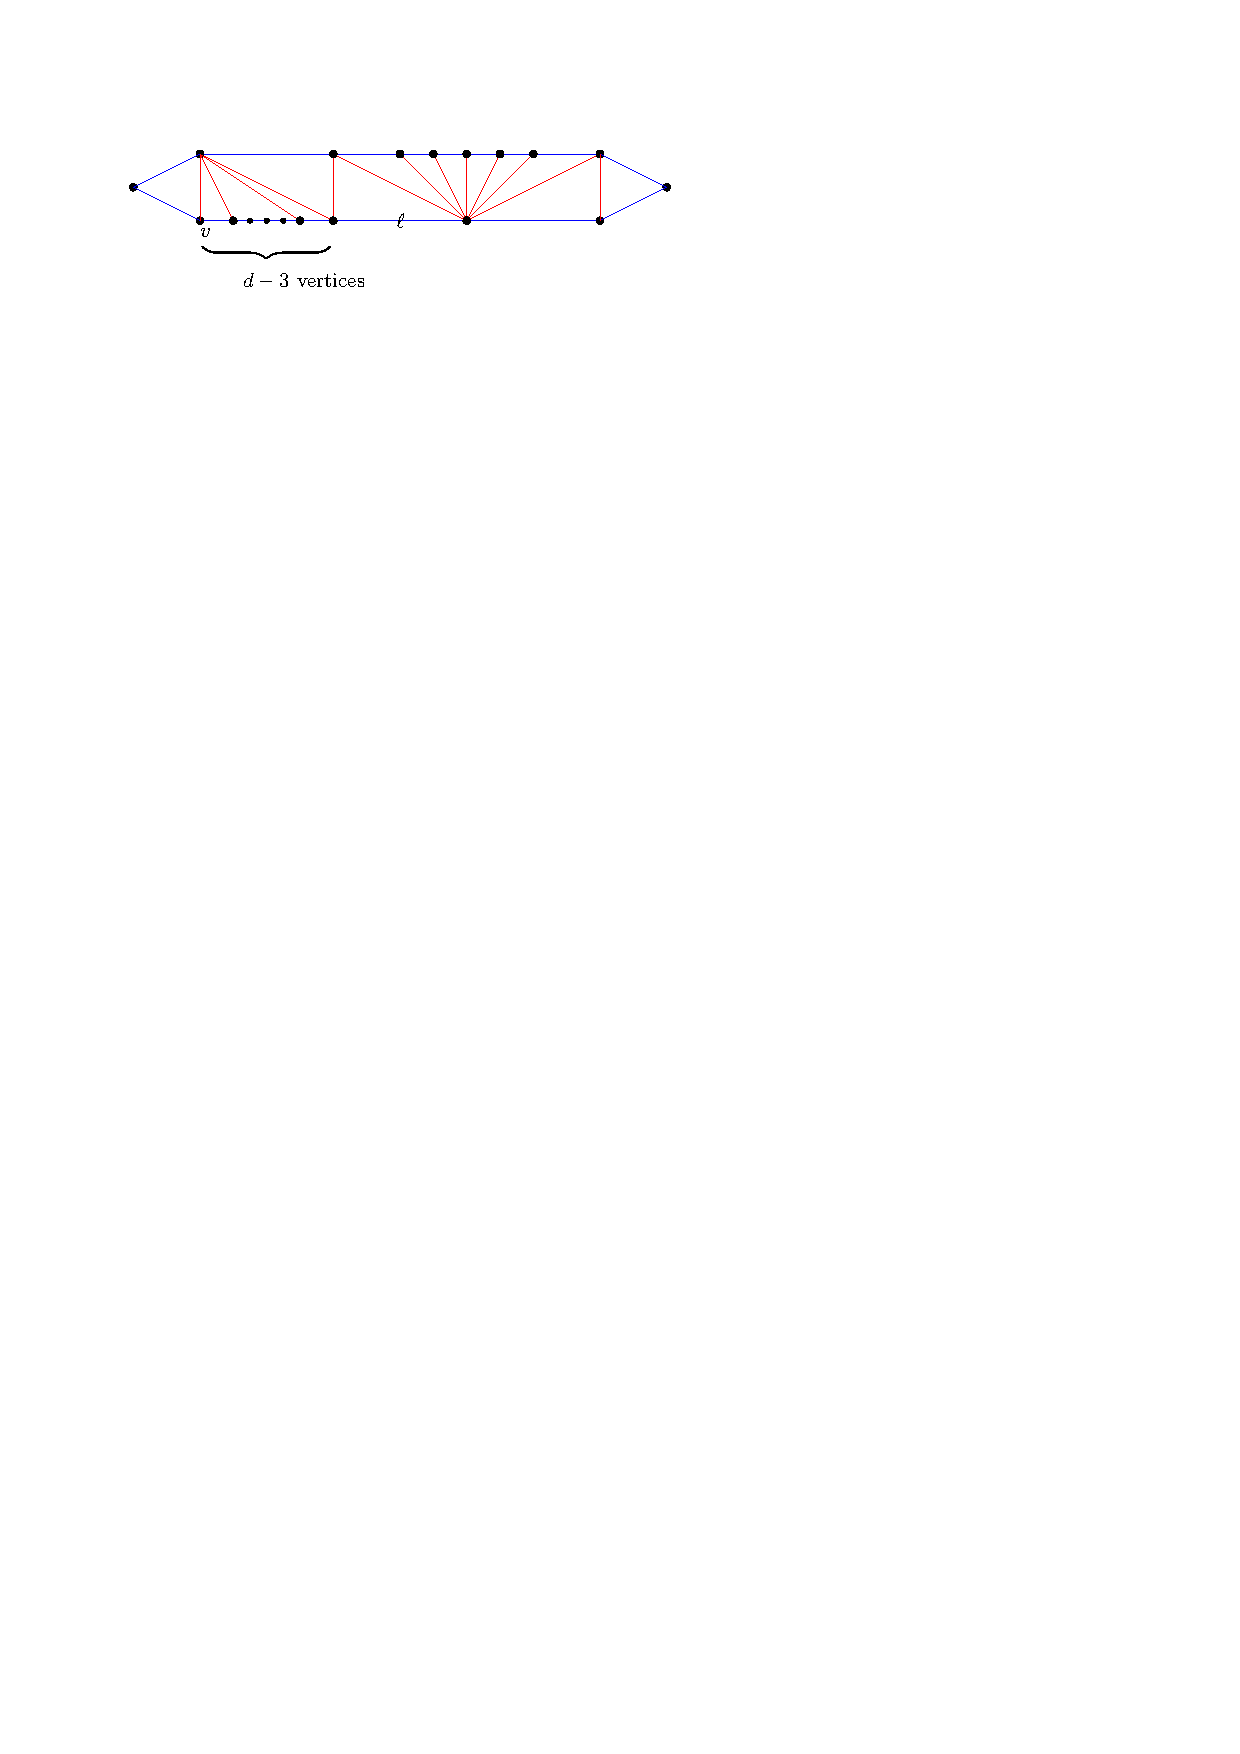
\includegraphics[scale=1]{blueFaceSubdivision/img/worstCaseWithTopFan}
    \caption{A worst case blue face. We do not flip any edge in this face.}
    \label{fig:subdiv:worstCaseWithTopFan}
  \end{figure}

  Note that we can flip to the right above each edge in the bottom boundary path except if we would end up next to the merge.

  We will look at the vertex on the bottom fence that is incident to the freshly flipped edge, or if we have not flipped an edge yet the vertex next to the split (and we denote it by $v$). The following are then the rules for flipping above the edges following $v$.
  \begin{enumerate}
    \item We do not flip above the edges of the first topfan.
    \item We flip above the second edge if it is unloaded.
    \item Otherwise, we flip above the third edge.
    \item We never flip next to the merge.
  \end{enumerate}

  When flipping above an edge, we always flip the right edge above that edge. Unless we are on the edge next to the merge, because then we flip the left edge above that edge.

  The first edge give us the required separation of loaded edges along the top boundary path. The other items make sure we obey the other rules.

  The worst case is given by a large topfan at the start and  a combination of the last two items. We would in that case want to flip above the second-to-last edge of the bottom boundary path. But we do not because the next edge is incident to the merge vertex. This gives at worst a topfan and  two more edges along the bottom boundary path and hence a $ d - 3 +2 = d -1$-sided face.
  \end{proof}

  See Figure \ref{fig:subdiv:sampleExecution} for a sample execution of the algorithm described in Lemma \ref{lm:subdiv:withoutTopfan}.

  \begin{figure}[t]
    \centering
    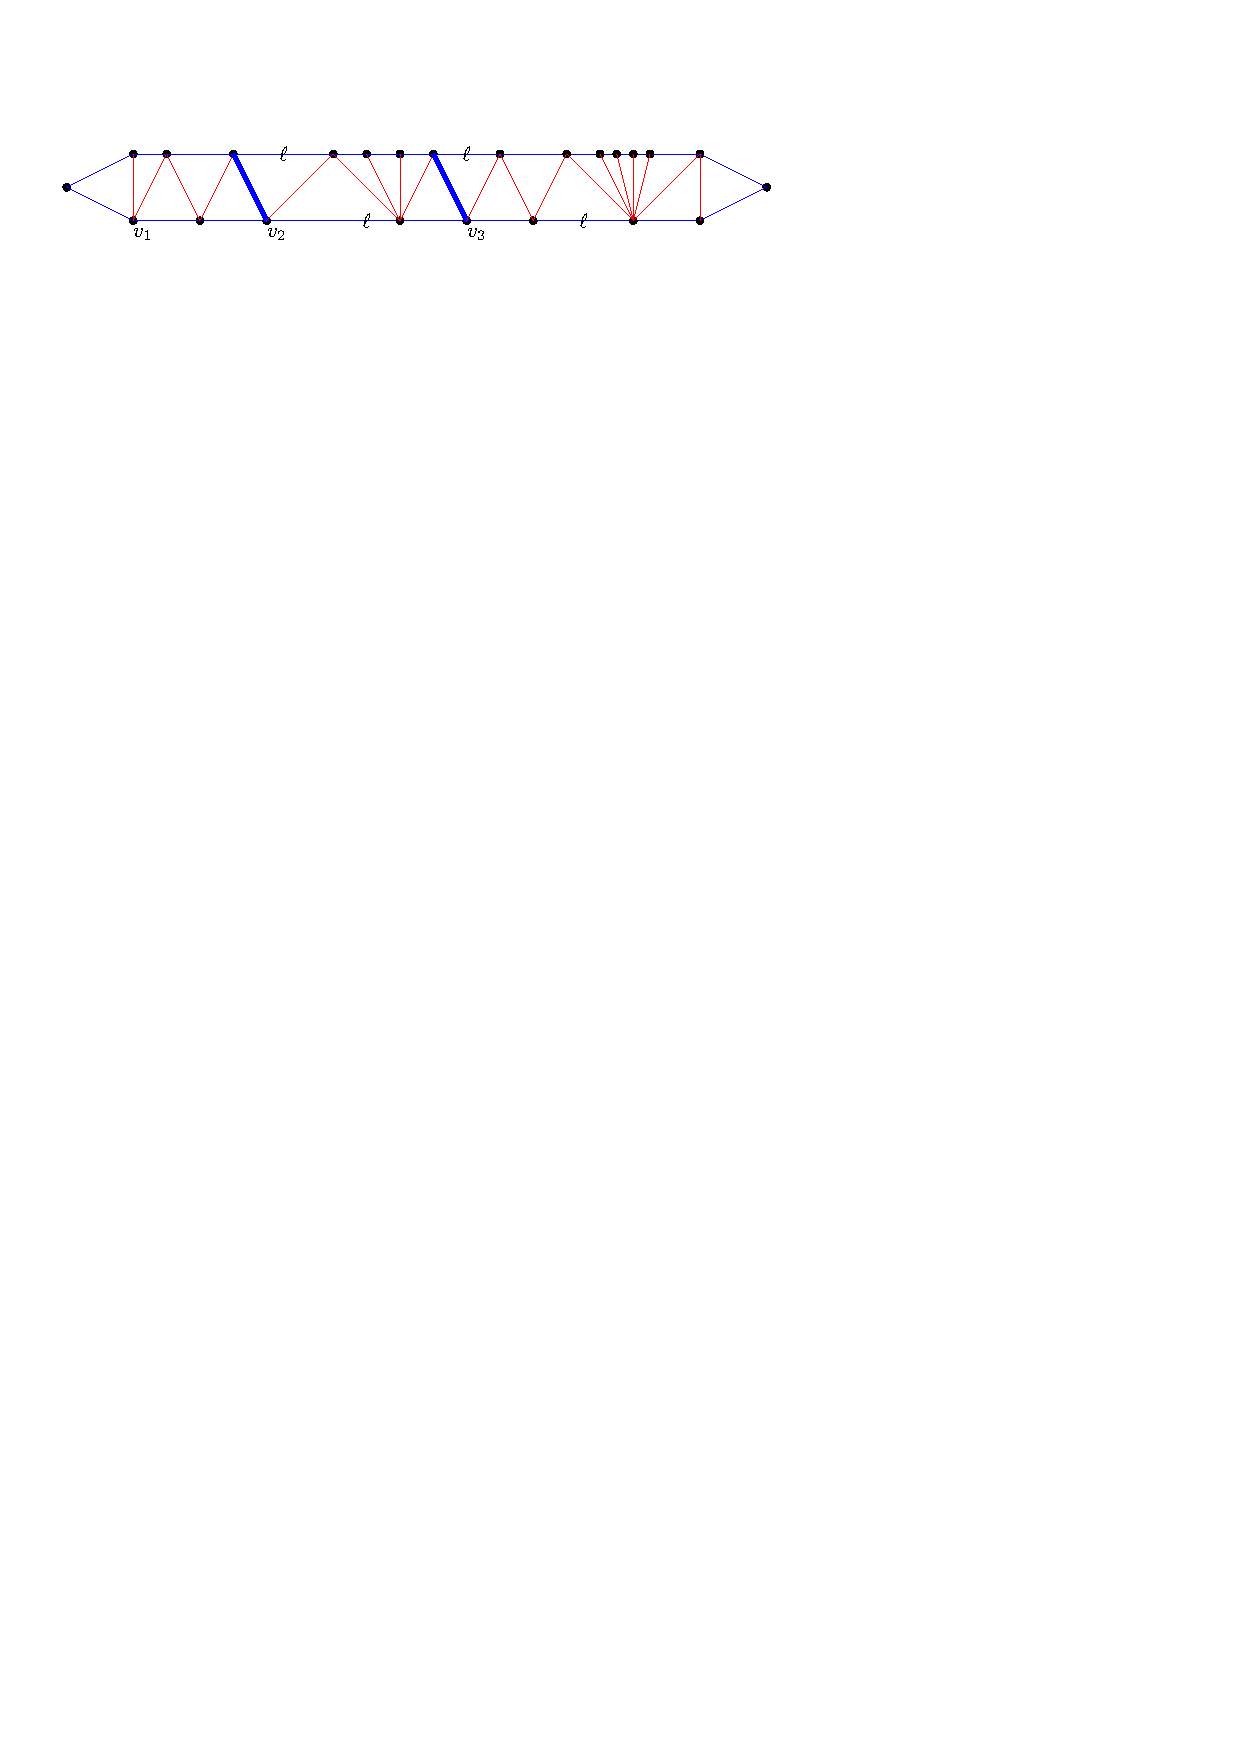
\includegraphics[scale=1]{blueFaceSubdivision/img/sampleExecution}
    \caption{Sample execution of the algorithm.}
    \label{fig:subdiv:sampleExecution}
  \end{figure}

\subsubsection{Face encountering a larger topfan}
  If we have a large topfan in the middle of the face then above the left outer edge of this topfan we can not, as we will see, have another topfan that failed to flip its left outer edges by Lemma \ref{lm:sweep:NoTwoSplitsAboveEachOther}.
  This means we can use the following rule: we flip the first edge of a topfan even above a loaded edge.
  We call such an edge a \emph{forced} flip.

  We can not have two such forced flips above each other because that would give a situation as in Figure \ref{fig:subdiv:forcedFlips}.
  However, that would mean the fan with fanhandle $u$ must be the handle of a topfan that failed its flip and hence $v$ must have been a split vertex. But then by lemma \ref{lm:zflip:NoTwoSplitsAboveEachOtherVertOnesided} $w$ can not be the handle of a large topfan.

  \begin{figure}[t]
    \centering
    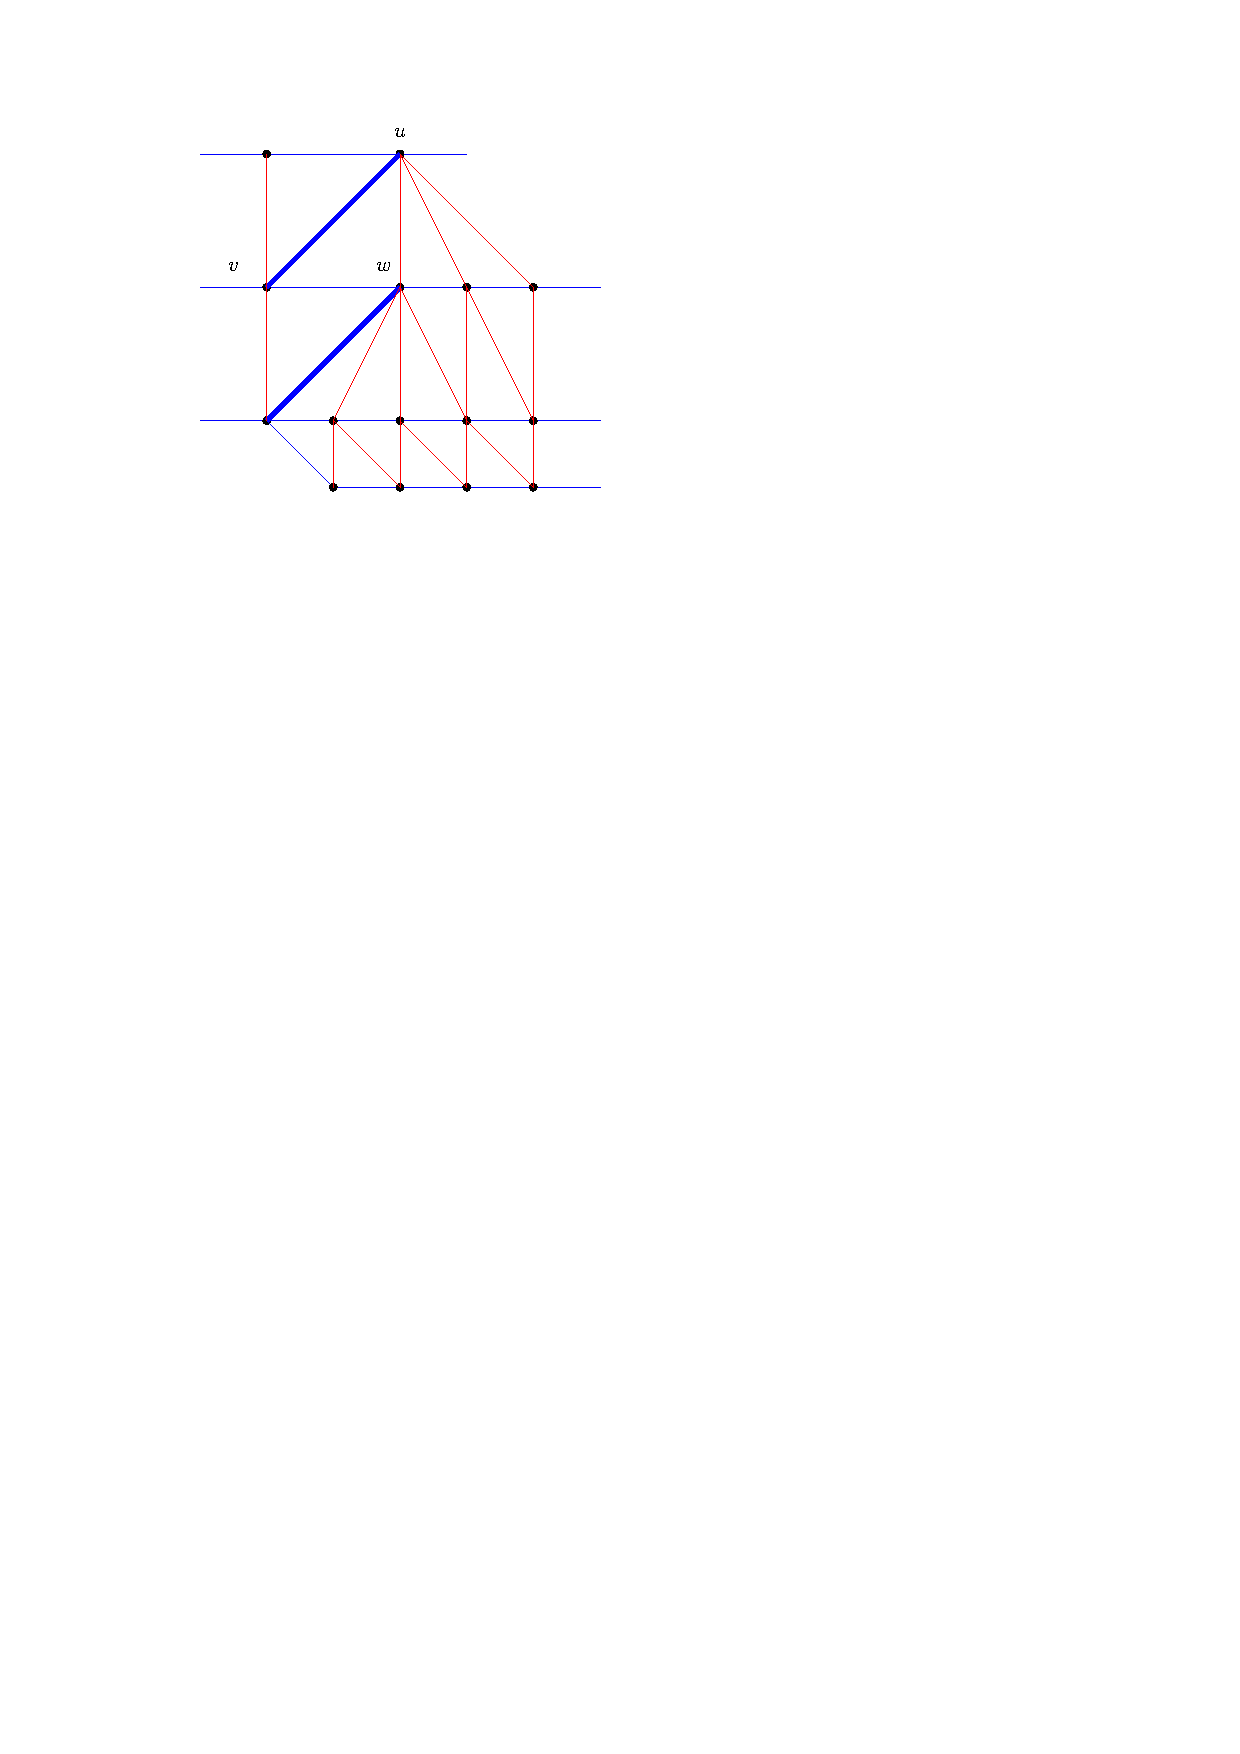
\includegraphics[scale=1]{blueFaceSubdivision/img/forcedFlips.pdf}
    \caption{Two forced flips above each other.}
    \label{fig:subdiv:forcedFlips}
  \end{figure}

  Since we do not allow a flip above a load (whether it was forced or not) this means that the worst thing that can happen is an ordinary flip followed by a \emph{forced} flip. These two flips can not be followed by any other flip. Hence, the worst case only makes chains of at most $2$ blue $Z$'s, that is, a blue path of length $5$.


\subsubsection{Conclusion}
  This concludes the last step in the algorithm.
  Now all the steps in the algorithm are done all that is left is to show that we indeed generated a $d-1$-sided regular edge labeling.
  \begin{lemma}
    \label{lm:subdiv:2chaindedZ}
    Two chained $Z$'s give at worst a red $d-1$-sided face
  \end{lemma}
  \begin{proof}
    %\fxwarning{TODO calrify, what are blue fans?}
    The two chained $Z$'s give a blue path $\P$ of length $5$ inside a red face.

    Before creating the $Z$'s in this section, the regular edge labeling was vertically one-sided.
    That is, before recoloring the two edges in this section there were no paths of length $3$ inside the face.
    This also implies that any $Z$ we now create can have at most one blue fan on the top and one blue fan on the bottom, otherwise we would already have had a $3$-path.

    So for two $Z$'s we have at most three blue fans.
    Hence, on one side we have at most one of these.
    Then the boundary path at this side of the face has at most $d-3 + 1 +1 =d-1$ vertices not counting the split and merge vertex of the red face.
  \end{proof}

    Then we can now prove Theorem \ref{th:dsided}.

  \begin{proof}[of Theorem \ref{th:dsided} ]
    By construction all blue faces are $d-1$-sided. We have chained at most two $Z's$ so all red face contain at most two blue $Z$. So red faces are $d-1$-sided by Lemma \ref{lm:subdiv:2chaindedZ}. Hence, we have a $d-1$-sided rectangular edge labeling of $\ext G$ corresponding to a $d$-sided rectangular dual of $\ext G$
  \end{proof}
